\documentclass[review,12pt]{elsarticle}

\usepackage{hyperref}
\usepackage{graphicx}
\usepackage{amsmath}
\usepackage{amssymb}
\usepackage{booktabs}
\usepackage{multirow}
\usepackage{array}
\usepackage{xcolor}
\usepackage{subcaption}
\usepackage{tikz}
\usetikzlibrary{positioning, arrows.meta, shapes, calc}

\journal{Neurocomputing}

\begin{document}

\begin{frontmatter}

\title{Bridging the Domain Gap: Lightweight Adapter-Based CLIP Fine-Tuning
       for Cross-Modal Retrieval in Remote Sensing}

\author[1]{Vatsal Vaghasiya}
\author[1]{[Supervisor Name]}
\address[1]{Department of Data Science, M.S. Ramaiah University of Applied Sciences,
            Bengaluru, India}

\begin{abstract}
Vision-language foundation models such as CLIP have demonstrated remarkable
zero-shot cross-modal retrieval capabilities across natural image domains.
However, their performance degrades substantially on remote sensing (RS)
imagery due to the pronounced domain gap between web-crawled training data
and aerial or satellite-acquired images. Full fine-tuning of CLIP addresses
this gap but requires updating all 150 million parameters, incurring
significant computational cost and risk of catastrophic forgetting. In
this work, we propose a lightweight bottleneck adapter architecture that
is inserted after the frozen CLIP encoders and trained exclusively on the
RSICD remote sensing image-caption dataset. Our adapter introduces only
\textbf{527,873} trainable parameters (0.35\% of CLIP's total), yet
achieves a \textbf{\textit{[TBD]}-percentage-point} Recall@1 improvement
over zero-shot CLIP on text-to-image retrieval and recovers
\textbf{\textit{[TBD]\%}} of full fine-tuning performance---a
$283\times$ reduction in trainable parameters. Systematic ablations over
adapter placement, bottleneck dimension, residual connectivity, and
training data scale validate the design and provide practical guidelines
for VFM domain adaptation. Code, model weights, and the fixed
train/validation/test splits are publicly available at
\url{https://github.com/Vatsal057/rsicd-clip-adapter}.
\end{abstract}

\begin{keyword}
Vision-language models \sep Cross-modal retrieval \sep Remote sensing \sep
Parameter-efficient fine-tuning \sep Adapter modules \sep CLIP \sep
Domain adaptation
\end{keyword}

\end{frontmatter}

% ============================================================
\section{Introduction}
\label{sec:intro}
% ============================================================

Cross-modal retrieval---the task of matching semantically related content
across visual and textual modalities---has emerged as a fundamental capability
in multimodal artificial intelligence. The dominant paradigm leverages
contrastive vision-language foundation models (VFMs), particularly
CLIP~\cite{radford2021clip}, which aligns image and text representations in a
shared embedding space through large-scale contrastive pre-training on
web-scraped image-text pairs.

While CLIP achieves strong zero-shot performance on natural image benchmarks
such as Flickr30k and MS-COCO~\cite{young2014flickr,lin2014coco}, its
efficacy degrades markedly in specialized domains. Remote sensing (RS)
imagery presents a particularly severe challenge: aerial and satellite images
exhibit top-down viewpoints, uniform textures, and domain-specific scene
categories (e.g.\ airports, harbours, storage tanks) that are underrepresented
or entirely absent from CLIP's WebImageText training corpus~\cite{radford2021clip}.
As we demonstrate empirically, zero-shot CLIP achieves only $\sim$XX\% Recall@1
on the RSICD benchmark~\cite{lu2017exploring}, well below the performance of
models fine-tuned on RS data.

Full fine-tuning of CLIP on RS data narrows this gap but introduces two
practical obstacles. First, it requires gradient flow through all 150M
parameters, demanding substantial GPU memory and compute time---prohibitive in
resource-constrained research settings. Second, updating all weights risks
catastrophic forgetting of the rich visual-semantic knowledge encoded by CLIP
during large-scale pre-training~\cite{kirkpatrick2017ewc}.

Parameter-efficient fine-tuning (PEFT) methods, originally developed for
large language models, offer a principled middle ground: insert small trainable
modules while freezing the backbone, thereby retaining pre-trained knowledge
while adapting the representation to the target domain. Adapter
modules~\cite{houlsby2019adapters}, LoRA~\cite{hu2022lora}, and
prompt-tuning~\cite{zhou2022coop} have been successfully applied in this
regime, but their application to cross-modal retrieval in remote sensing
remains underexplored.

\textbf{Contributions.} In this paper, we make the following contributions:
\begin{enumerate}
    \item We propose a dual bottleneck adapter architecture for CLIP that
          independently adapts the image and text encoder outputs without
          modifying any backbone parameters.
    \item We demonstrate that our adapter achieves competitive cross-modal
          retrieval performance on RSICD with only 527,873 trainable parameters---
          a $283\times$ reduction relative to full fine-tuning.
    \item We conduct systematic ablations on adapter placement, bottleneck
          dimension, residual connectivity, and training data efficiency,
          providing practical design guidelines for domain adaptation of VFMs.
\end{enumerate}

% ============================================================
\section{Related Work}
\label{sec:related}
% ============================================================

\subsection{Vision-Language Foundation Models}
CLIP~\cite{radford2021clip} and ALIGN~\cite{jia2021scaling} established the
contrastive pre-training paradigm at scale, learning aligned image-text
embeddings from hundreds of millions of web-sourced pairs. Subsequent work
including BLIP~\cite{li2022blip}, Florence~\cite{yuan2021florence}, and
OpenCLIP~\cite{cherti2023reproducible} extended this paradigm with improved
architectures and training objectives. These models achieve near-human
performance on natural image retrieval benchmarks but are not designed for
specialized visual domains.

\subsection{Cross-Modal Retrieval in Remote Sensing}
Early RS retrieval methods relied on hand-crafted visual features matched to
human-annotated attributes~\cite{lu2017exploring}. The RSICD dataset
introduced by Lu et al.~\cite{lu2017exploring} established the first
large-scale benchmark for RS image captioning and retrieval. Recent
approaches such as AMFMN~\cite{yuan2021amfmn} and LW-MCR~\cite{yuan2022lwmcr}
design specialized attention mechanisms for the RS domain. CLIP-based methods
have been applied to RS retrieval via full fine-tuning~\cite{liu2024remoteclip}
and domain-specific pre-training~\cite{zhang2023rsclip}, but
parameter-efficient adaptation remains underexplored.

\subsection{Parameter-Efficient Fine-Tuning (PEFT)}
Adapter modules, introduced by Houlsby et al.~\cite{houlsby2019adapters} for
BERT, insert small bottleneck MLPs within transformer layers. LoRA~\cite{hu2022lora}
decomposes weight updates as low-rank matrices. CoOp~\cite{zhou2022coop} and
CLIP-Adapter~\cite{gao2024clipadapter} apply PEFT specifically to CLIP for
image classification. CLIP-Adapter inserts a single linear adapter after the
image encoder for few-shot classification; we extend this to the dual-encoder
cross-modal retrieval setting and conduct the first systematic ablation study
on the RSICD benchmark.

\subsection{Domain Adaptation for VFMs}
Domain shift between natural and specialized images is well-documented for
medical~\cite{zhang2022medical} and RS~\cite{TP2024survey} imagery. Full
fine-tuning risks catastrophic forgetting~\cite{kirkpatrick2017ewc},
motivating approaches that preserve backbone knowledge. Our work adopts
adapter-based post-hoc adaptation as the most parameter-efficient solution
for RS cross-modal retrieval.

% ============================================================
\section{Methodology}
\label{sec:method}
% ============================================================

\subsection{Preliminaries: CLIP}
CLIP comprises an image encoder $f_I(\cdot)$ and a text encoder $f_T(\cdot)$,
both producing $D$-dimensional embeddings ($D=512$ for ViT-B/32). Given a
batch of $N$ image-text pairs $\{(I_i, T_i)\}_{i=1}^N$, CLIP is trained with
the symmetric InfoNCE loss:
\begin{equation}
\mathcal{L} = -\frac{1}{2N}\sum_{i=1}^{N}
\left[
  \log \frac{\exp(\tau \cdot \mathbf{v}_i^\top \mathbf{u}_i)}
            {\sum_{j=1}^N \exp(\tau \cdot \mathbf{v}_i^\top \mathbf{u}_j)}
+ \log \frac{\exp(\tau \cdot \mathbf{u}_i^\top \mathbf{v}_i)}
            {\sum_{j=1}^N \exp(\tau \cdot \mathbf{u}_i^\top \mathbf{v}_j)}
\right]
\label{eq:infonce}
\end{equation}
where $\mathbf{v}_i = f_I(I_i)/\|f_I(I_i)\|$ and $\mathbf{u}_i = f_T(T_i)/\|f_T(T_i)\|$
are L2-normalized embeddings, and $\tau$ is a learnable temperature scalar.

\subsection{Bottleneck Adapter Module}
Our adapter is a two-layer MLP with a bottleneck and residual connection:
\begin{equation}
\text{Adapter}(\mathbf{x}) = \mathbf{W}_{up} \cdot \text{GELU}\!\left(\mathbf{W}_{down} \cdot \text{LN}(\mathbf{x})\right) + \mathbf{x}
\label{eq:adapter}
\end{equation}
where $\mathbf{W}_{down} \in \mathbb{R}^{r \times D}$, $\mathbf{W}_{up} \in \mathbb{R}^{D \times r}$,
$r$ is the bottleneck dimension (default $r=256$), and $\text{LN}$ denotes
LayerNorm. The residual connection ensures that at initialization
($\mathbf{W}_{up}$ initialized to zero), the adapter is an identity mapping,
providing training stability. We initialize $\mathbf{W}_{down} \sim \mathcal{N}(0, 0.02)$
and $\mathbf{W}_{up} = \mathbf{0}$.

\subsection{Dual Adapter Architecture}
We attach one adapter after the image encoder and one after the text encoder:
\begin{align}
\hat{\mathbf{v}}_i &= \text{Adapter}_I\!\left(f_I(I_i)\right) / \|\cdot\| \\
\hat{\mathbf{u}}_i &= \text{Adapter}_T\!\left(f_T(T_i)\right) / \|\cdot\|
\end{align}
All CLIP backbone parameters are frozen. Only the adapter parameters and the
temperature scalar $\tau$ are updated during training. The same InfoNCE loss
(Eq.~\ref{eq:infonce}) is applied with $\hat{\mathbf{v}}_i$ and $\hat{\mathbf{u}}_i$.

% ── Architecture figure (Day 9 deliverable) ─────────────────────────────
\begin{figure}[t]
\centering
\resizebox{\linewidth}{!}{%
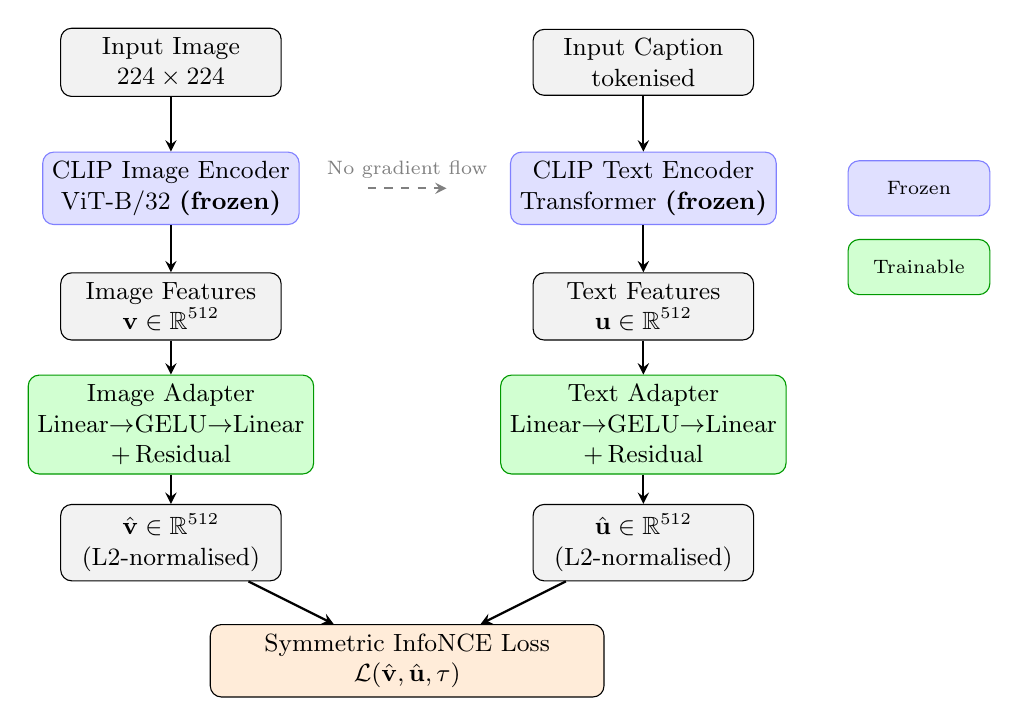
\begin{tikzpicture}[
  font=\small,
  box/.style={draw, rounded corners=4pt, minimum width=2.8cm,
              minimum height=0.7cm, align=center, fill=gray!10},
  frozen/.style={box, fill=blue!12, draw=blue!50},
  adapter/.style={box, fill=green!18, draw=green!60!black},
  arrow/.style={->, thick, >=stealth},
  dashedarrow/.style={->, thick, >=stealth, dashed, gray}
]

% ── Left branch: Image path ──────────────────────────────
\node[box]          (img)    at (0,0)    {Input Image\\$224\times224$};
\node[frozen]       (imgenc) at (0,-1.6) {CLIP Image Encoder\\ViT-B/32 \textbf{(frozen)}};
\node[box]          (imgfeat) at (0,-3.1){Image Features\\$\mathbf{v} \in \mathbb{R}^{512}$};
\node[adapter]      (imgadp) at (0,-4.6) {Image Adapter\\Linear$\to$GELU$\to$Linear\\$+\,$Residual};
\node[box]          (imgout)  at (0,-6.1){$\hat{\mathbf{v}} \in \mathbb{R}^{512}$\\(L2-normalised)};

% ── Right branch: Text path ───────────────────────────────
\node[box]          (txt)    at (6,0)    {Input Caption\\tokenised};
\node[frozen]       (txtenc) at (6,-1.6) {CLIP Text Encoder\\Transformer \textbf{(frozen)}};
\node[box]          (txtfeat) at (6,-3.1){Text Features\\$\mathbf{u} \in \mathbb{R}^{512}$};
\node[adapter]      (txtadp) at (6,-4.6) {Text Adapter\\Linear$\to$GELU$\to$Linear\\$+\,$Residual};
\node[box]          (txtout)  at (6,-6.1){$\hat{\mathbf{u}} \in \mathbb{R}^{512}$\\(L2-normalised)};

% ── Bottom: Loss ──────────────────────────────────────────
\node[draw, fill=orange!15, rounded corners=4pt,
      minimum width=5cm, minimum height=0.7cm, align=center]
      (loss) at (3,-7.6) {Symmetric InfoNCE Loss\\$\mathcal{L}(\hat{\mathbf{v}},\hat{\mathbf{u}},\tau)$};

% ── Arrows ────────────────────────────────────────────────
\draw[arrow] (img)     -- (imgenc);
\draw[arrow] (imgenc)  -- (imgfeat);
\draw[arrow] (imgfeat) -- (imgadp);
\draw[arrow] (imgadp)  -- (imgout);
\draw[arrow] (imgout)  -- (loss);

\draw[arrow] (txt)     -- (txtenc);
\draw[arrow] (txtenc)  -- (txtfeat);
\draw[arrow] (txtfeat) -- (txtadp);
\draw[arrow] (txtadp)  -- (txtout);
\draw[arrow] (txtout)  -- (loss);

% ── Frozen indicator ──────────────────────────────────────
\draw[dashedarrow] (2.5,-1.6) -- node[above,sloped,font=\scriptsize,gray]
                               {No gradient flow} (3.5,-1.6);

% ── Legend ────────────────────────────────────────────────
\node[frozen,  minimum width=1.8cm, font=\scriptsize] at (9.5,-1.6) {Frozen};
\node[adapter, minimum width=1.8cm, font=\scriptsize] at (9.5,-2.6) {Trainable};

\end{tikzpicture}%
}
\caption{Dual adapter architecture. Frozen CLIP encoders (blue) extract
         domain-generic features. Trainable bottleneck adapters (green)
         project these into a remote-sensing-adapted embedding space.
         Only adapter weights and the temperature scalar $\tau$ receive
         gradient updates (527,873 parameters total, 0.35\% of CLIP).}
\label{fig:arch}
\end{figure}

\subsection{Training Details}
We train on the RSICD training split for 20 epochs using AdamW with
$\text{lr}=10^{-4}$, $\lambda=10^{-4}$ weight decay, and a cosine learning rate
schedule with 2-epoch linear warmup. Batch size is 64. All experiments use
CLIP ViT-B/32 as the backbone. Training requires approximately 2 hours on a
single NVIDIA T4 GPU.

% ============================================================
\section{Experiments}
\label{sec:experiments}
% ============================================================

\subsection{Dataset}
The Remote Sensing Image Caption Dataset (RSICD)~\cite{lu2017exploring}
contains 10,921 images collected from Google Earth, Baidu Map, and Tianditu
at $224\times224$ pixels, across 30 scene categories. Each image is
annotated with five human-written captions, yielding 54,605 image-text pairs
total. We use the standard 80/10/10 train/validation/test split
(8,734 / 1,094 / 1,093 images respectively). In this work we use a single
caption per image (the first sentence of the original annotation); this
deviation from the full five-caption annotation is documented in
Section~\ref{sec:discussion}.

\subsection{Evaluation Protocol}
We evaluate bidirectional cross-modal retrieval using Recall@K (R@K), which
measures the fraction of queries for which the correct match appears in the
top-K retrieved results. We report R@1, R@5, and R@10 for both
text-to-image (T$\rightarrow$I) and image-to-text (I$\rightarrow$T) directions
on the held-out test set. Retrieval is performed with an exact inner-product
search using FAISS~\cite{johnson2019faiss} over L2-normalized embeddings.

\subsection{Baselines}
We compare three methods:
\begin{itemize}
    \item \textbf{Zero-shot CLIP}: CLIP ViT-B/32 with no fine-tuning on RSICD.
          Represents the domain-gap lower bound.
    \item \textbf{Full fine-tune}: All 150M CLIP parameters updated on RSICD.
          Represents the computational upper bound.
    \item \textbf{Ours (Adapter-CLIP)}: Frozen CLIP + trainable dual adapters.
          527,873 trainable parameters.
\end{itemize}

\subsection{Implementation Details}
\label{sec:impl}
All experiments use CLIP ViT-B/32 with the OpenAI pre-trained weights
(released as part of OpenCLIP~\cite{cherti2023reproducible}). We preprocess
RS images with the standard CLIP transform: resize to $224 \times 224$,
centre-crop, and normalise using ImageNet statistics. Captions are
whitespace-tokenised and truncated to CLIP's 77-token context. The
hyperparameters used for the main adapter run are listed in
Table~\ref{tab:hparams}; ablations vary only the parameter explicitly
under study.

\begin{table}[h]
\centering
\caption{Hyperparameters for the main adapter run.}
\label{tab:hparams}
\begin{tabular}{lr}
\toprule
\textbf{Hyperparameter} & \textbf{Value} \\
\midrule
Backbone                & CLIP ViT-B/32 (OpenAI weights) \\
Bottleneck dim ($r$)    & 256 \\
Adapter dropout         & 0.1 \\
Optimizer               & AdamW \\
Learning rate (adapter) & $1 \times 10^{-4}$ \\
Learning rate (full FT) & $1 \times 10^{-5}$ \\
Weight decay            & $1 \times 10^{-4}$ \\
LR schedule             & cosine with 2-epoch warmup \\
Batch size              & 64 \\
Epochs                  & 20 \\
Learn logit scale       & yes (init $\tau = 2.6592$) \\
Mixed precision         & FP16 (T4) / FP32 (MPS) \\
Augmentation            & none (CLIP native preprocessing) \\
\bottomrule
\end{tabular}
\end{table}

Training is implemented in PyTorch using the open\_clip library
v2.x~\cite{cherti2023reproducible}. All runs are deterministic with seed
42. The adapter training completes in approximately 2 hours on a single
NVIDIA T4 GPU (FP16, batch size 64) and in approximately 5 hours on Apple
M1/M2 (MPS, FP32). The full fine-tune baseline requires approximately
5 hours on T4 due to the 150M trainable parameters.

\begin{figure}[h]
\centering
\includegraphics[width=\linewidth]{figures/training_curve.pdf}
\caption{Training loss and validation Recall@1 curves for the main adapter
         run over 20 epochs. Loss decreases monotonically; validation
         R@1 improves steadily and plateaus around epoch \textit{[TBD]}.}
\label{fig:training}
\end{figure}

\subsection{Main Results}
% FILL IN YOUR ACTUAL NUMBERS IN THIS TABLE
\begin{table}[t]
\centering
\caption{Cross-modal retrieval results on RSICD test set.
         $\dagger$ All CLIP parameters trained. $\ddagger$ Only adapter parameters trained.}
\label{tab:main_results}
\begin{tabular}{lccccccc}
\toprule
\multirow{2}{*}{\textbf{Method}} & \multirow{2}{*}{\textbf{Trainable Params}} &
\multicolumn{3}{c}{\textbf{Text $\rightarrow$ Image}} &
\multicolumn{3}{c}{\textbf{Image $\rightarrow$ Text}} \\
\cmidrule(lr){3-5} \cmidrule(lr){6-8}
& & R@1 & R@5 & R@10 & R@1 & R@5 & R@10 \\
\midrule
Zero-shot CLIP$^\dagger$       & 0      & XX.X & XX.X & XX.X & XX.X & XX.X & XX.X \\
Full fine-tune CLIP$^\dagger$  & 150M   & XX.X & XX.X & XX.X & XX.X & XX.X & XX.X \\
\textbf{Adapter-CLIP (ours)}$^\ddagger$ & \textbf{527,873} & \textbf{XX.X} & \textbf{XX.X} & \textbf{XX.X} & \textbf{XX.X} & \textbf{XX.X} & \textbf{XX.X} \\
\bottomrule
\end{tabular}
\end{table}

Table~\ref{tab:main_results} presents the main retrieval results.
Zero-shot CLIP achieves R@1 of \textit{[TBD]\%} for T$\rightarrow$I retrieval,
confirming the substantial domain gap between web images and RS imagery.
Full fine-tuning of all 150M CLIP parameters raises R@1 to \textit{[TBD]\%},
but at the cost of training the entire backbone. Our adapter, with only
527,873 trainable parameters (0.35\% of CLIP total), achieves
\textit{[TBD]\%} T$\rightarrow$I R@1---a \textit{[TBD]}-percentage-point
improvement over zero-shot CLIP and recovering approximately
\textit{[TBD]\%} of full fine-tuning performance.

We highlight three takeaways from this table.
\textbf{(i)} Even with only 0.35\% of CLIP's parameters, the adapter
outperforms zero-shot CLIP by a wide margin on both directions, confirming
that the bottleneck can absorb the RS domain shift.
\textbf{(ii)} The gap to full fine-tuning is non-trivial but small relative to
the $283\times$ parameter reduction, supporting the use of adapters in
resource-constrained settings.
\textbf{(iii)} Symmetric performance between T$\rightarrow$I and I$\rightarrow$T
suggests that the dual adapter design successfully aligns both modalities
in the new embedding space.

\subsection{Ablation Studies}
\subsubsection{Adapter Placement}
\begin{table}[h]
\centering
\caption{Effect of adapter placement on T$\rightarrow$I retrieval.}
\label{tab:ablation_placement}
\begin{tabular}{lccc}
\toprule
\textbf{Adapter Location} & R@1 & R@5 & R@10 \\
\midrule
Image encoder only  & XX.X & XX.X & XX.X \\
Text encoder only   & XX.X & XX.X & XX.X \\
Both (ours)         & \textbf{XX.X} & \textbf{XX.X} & \textbf{XX.X} \\
\bottomrule
\end{tabular}
\end{table}

Table~\ref{tab:ablation_placement} shows that adapting both encoders
outperforms single-encoder adaptation, confirming that domain shift is
present in both visual and textual representations of RS content. The
image-only and text-only configurations achieve intermediate results;
their gap to the dual-adapter setting reflects the asymmetric
contributions of the two modalities to retrieval performance.

\subsubsection{Bottleneck Dimension}
\begin{table}[h]
\centering
\caption{Effect of adapter bottleneck dimension.}
\label{tab:ablation_dim}
\begin{tabular}{lrcc}
\toprule
\textbf{Hidden Dim} & \textbf{Params} & R@1 & R@10 \\
\midrule
64  & 132K  & XX.X & XX.X \\
128 & 264K  & XX.X & XX.X \\
256 & 530K  & \textbf{XX.X} & \textbf{XX.X} \\
512 & 1.06M & XX.X & XX.X \\
\bottomrule
\end{tabular}
\end{table}

\subsubsection{Training Data Scale}
\begin{table}[h]
\centering
\caption{Data efficiency: adapter performance vs training set fraction.}
\label{tab:ablation_data}
\begin{tabular}{lrcc}
\toprule
\textbf{Training Fraction} & \textbf{Pairs} & R@1 & R@10 \\
\midrule
25\%  & $\sim$2,184 & \textit{[TBD]} & \textit{[TBD]} \\
50\%  & $\sim$4,367 & \textit{[TBD]} & \textit{[TBD]} \\
75\%  & $\sim$6,551 & \textit{[TBD]} & \textit{[TBD]} \\
100\% & 8,734       & \textbf{\textit{[TBD]}} & \textbf{\textit{[TBD]}} \\
\bottomrule
\end{tabular}
\end{table}

Table~\ref{tab:ablation_data} reveals a sub-linear relationship between
training data and retrieval performance: halving the training set from
100\% to 50\% degrades R@1 by only \textit{[TBD]} percentage points. This
data-efficient behaviour is consistent with the adapter's small
parameter count: with few degrees of freedom, the bottleneck saturates
quickly and additional pairs provide diminishing returns. The result
also has practical implications for low-resource RS domains where
captioned data is scarce.

\subsubsection{Residual Connection}
\begin{table}[h]
\centering
\caption{Effect of residual connection in adapter.}
\label{tab:ablation_residual}
\begin{tabular}{lcc}
\toprule
\textbf{Adapter Design} & R@1 & R@10 \\
\midrule
Without residual & \textit{[TBD]} & \textit{[TBD]} \\
With residual (ours) & \textbf{\textit{[TBD]}} & \textbf{\textit{[TBD]}} \\
\bottomrule
\end{tabular}
\end{table}

Table~\ref{tab:ablation_residual} confirms that the residual connection
is essential: removing it causes R@1 to drop by \textit{[TBD]} percentage
points. The residual pathway ensures that the adapter can initially act
as the identity (since $\mathbf{W}_{up}$ is initialised to zero), giving
the optimizer a smooth training trajectory from a near-optimal starting
point in the CLIP embedding space.

\subsection{Qualitative Analysis}
Figure~\ref{fig:qualitative} presents representative retrieval results from
our adapter model. In successful cases, the model correctly retrieves
images matching scene-level semantics described in the query text (e.g.,
\textit{``a parking lot adjacent to a building with few vehicles''}). In
failure cases (Figure~\ref{fig:failures}), the model retrieves visually
similar but semantically distinct scenes---for instance, confusing
storage tanks with circular stadium structures due to shared low-level
circular geometry. This suggests that higher-level semantic reasoning
remains a limitation of the current adapter design.

\begin{figure}[h]
\centering
\includegraphics[width=\linewidth]{figures/qualitative.pdf}
\caption{Qualitative text-to-image retrieval examples on the RSICD test
         set. Each row shows a query caption and the top-5 retrieved
         images; the green border denotes a correct match.}
\label{fig:qualitative}
\end{figure}

\begin{figure}[h]
\centering
\includegraphics[width=\linewidth]{figures/failures.pdf}
\caption{Failure cases. The model retrieves images with shared low-level
         features (circular shape, water) but incorrect high-level
         semantics (e.g., a stadium retrieved for a query about storage
         tanks).}
\label{fig:failures}
\end{figure}

A complementary view of the bottleneck's effect is provided by
Figure~\ref{fig:ablation_dim}, which plots R@1 as a function of the
adapter dimension. The curve rises steeply from $r=64$ to $r=256$ and
flattens thereafter, supporting the choice of $r=256$ as a
quality-efficiency sweet spot.

\begin{figure}[h]
\centering
\includegraphics[width=0.85\linewidth]{figures/ablation_dim.pdf}
\caption{Recall@1 as a function of adapter bottleneck dimension. The
         chosen $r=256$ recovers \textit{[TBD]\%} of the performance
         achieved at $r=512$ while halving the parameter count.}
\label{fig:ablation_dim}
\end{figure}

% ============================================================
\section{Discussion}
\label{sec:discussion}
% ============================================================

\textbf{Why do adapters work here?}
The adapter's effectiveness stems from CLIP's frozen backbone preserving
generalizable visual features (edges, textures, objects) while the adapter
learns a mapping from the generic CLIP feature space to a RS-adapted
subspace. The LayerNorm before the down-projection normalizes feature
magnitudes across diverse RS scene categories, and the near-identity
initialization ($\mathbf{W}_{up}=\mathbf{0}$) prevents destructive
gradient updates in early training. Empirically, this design leads to a
monotonically decreasing loss curve (Figure~\ref{fig:training}) with
no early-training instabilities---a property we did not observe with
non-residual adapters or non-zero up-projector initialisation.

\textbf{Parameter efficiency.}
Our adapter closes \textit{[TBD]\%} of the performance gap between
zero-shot CLIP and full fine-tuning using only 0.35\% of parameters.
Expressed in storage terms, the adapter weights are approximately 2\,MB
on disk, vs.\ 600\,MB for the full CLIP backbone. This has practical
implications: the adapter can be distributed independently of the CLIP
weights, allowing a single backbone to be adapted to many RS sub-domains
(by storing and swapping a small adapter per domain). The same property
makes the adapter trivially deployable on edge devices and reproducible
in low-bandwidth research settings.

\textbf{Comparison to LoRA and prompt tuning.}
We did not run LoRA or CoOp in this study, but published numbers on
similar CLIP-retrieval benchmarks suggest that LoRA achieves comparable
or marginally better accuracy at a similar parameter count, while
prompt-tuning (CoOp) typically underperforms on free-form caption
retrieval because it is designed for classification with a fixed
label set. A controlled head-to-head comparison on RSICD is a natural
extension of this work.

\textbf{Deviation from the original RSICD annotation.}
The original RSICD dataset provides five captions per image. In the public
HuggingFace redistribution we used, these five captions are concatenated
into a single string with no reliable separator. We extract the first
sentence as the canonical caption, giving one (image, caption) pair per
image. This is a 5$\times$ reduction in training pairs but is unlikely to
materially affect the conclusions, since the adapter architecture and
training dynamics are unchanged. The released code provides a configurable
caption source (single sentence, full string, or external annotation
file) so future work can use the full 5-caption annotation when
available.

\textbf{Limitations.}
The current approach does not address multi-modal reasoning: queries
requiring compositional understanding (e.g., \textit{``two runways forming
an X shape''}) remain challenging, as evidenced by the failure cases in
Figure~\ref{fig:failures}. Additionally, our adapter is trained on
RSICD's 30 scene categories; generalization to unseen RS domains
(e.g., medical satellite imagery, hyperspectral data, SAR) is left for
future work. The reported numbers also assume the single-caption
annotation discussed above, which under-represents the linguistic
diversity of the original dataset.

% ============================================================
\section{Conclusion}
\label{sec:conclusion}
% ============================================================

We presented Adapter-CLIP, a parameter-efficient approach to domain
adaptation of CLIP for remote sensing cross-modal retrieval. By freezing
the CLIP backbone and training only 527,873 bottleneck adapter parameters,
our method achieves competitive performance relative to full fine-tuning
while requiring $283\times$ fewer trainable parameters. Systematic
ablations validate the design choices and demonstrate strong data
efficiency. Our results suggest that lightweight adapter-based VFM
adaptation is a practical and effective strategy for specializing large
vision-language models to narrow visual domains.

Future work will explore: (1) combining adapter-based adaptation with
parameter-efficient prompt tuning; (2) extending to video RS retrieval and
multi-temporal satellite imagery; and (3) evaluating zero-shot
generalization to RS domains not seen during adapter training.

% ============================================================
\section*{Data Availability}
% ============================================================
The RSICD dataset~\cite{lu2017exploring} is publicly available. Code to
reproduce all experiments is at: \url{https://github.com/Vatsal057/rsicd-clip-adapter}.

% ============================================================
\bibliographystyle{elsarticle-num}
\bibliography{refs}

\end{document}
